\documentclass[8pt]{beamer} %with breakpoints
%\documentclass[8pt,handout]{beamer} %no breakpoints
\usetheme{Madrid}

\usepackage[utf8]{inputenc}
\usepackage{amsmath}
\usepackage{amssymb}
\usepackage{enumerate}
%\usepackage{mathpazo}
\usepackage{relsize}
\usepackage{mathtools}
\usepackage{verbatim}

\usepackage{tikz}
\usetikzlibrary{matrix,arrows}

\usepackage{commands}

\setbeamertemplate{navigation symbols}{}%remove navigation symbols
%\setbeamertemplate{frametitle}[default][center]
\makeatletter
\setbeamertemplate{footline}
{
  \leavevmode%
  \hbox{%
  \begin{beamercolorbox}[wd=.35\paperwidth,ht=2.25ex,dp=1ex,center]{author in head/foot}%
    \usebeamerfont{author in head/foot}\insertshortauthor\expandafter\beamer@ifempty\expandafter{\beamer@shortinstitute}{}{~~(\insertshortinstitute)}
  \end{beamercolorbox}%
  \begin{beamercolorbox}[wd=.45\paperwidth,ht=2.25ex,dp=1ex,center]{title in head/foot}%
    \usebeamerfont{title in head/foot}\insertshorttitle
  \end{beamercolorbox}%
  \begin{beamercolorbox}[wd=.2\paperwidth,ht=2.25ex,dp=1ex,right]{date in head/foot}%
    \usebeamerfont{date in head/foot}\insertshortdate{}\hspace*{2em}
\insertframenumber{} / \inserttotalframenumber\hspace*{2ex} 
  \end{beamercolorbox}}%
  \vskip0pt%
}
\makeatother



\title{Uhlenbeck compactification as a Bridgeland moduli space}
%\subtitle{Determinantal line bundles on moduli of complexes}
\author{Tuomas Tajakka}
\institute{University of Washington}
\date{October 28, 2020}


\begin{document}

\begin{frame}
    \titlepage
\end{frame}

\begin{frame}{Outline}
    \tableofcontents    
\end{frame}

\section{Dimension 1}
\subsection{Slope stability on a curve}
\begin{frame}[fragile]{Dim 1: Slope stability on a curve}
\begin{columns}[t]
    \column{0.5\textwidth}
    \begin{itemize}
        \item<2-> $C$ a smooth, projective curve over $\C$
        \item<3-> (everything will be over $\C$ - for safety)
        \item<4-> \textbf{Slope} of $E \in \Coh(C)$:
        \[ \mu(E) = \frac{\deg(E)}{\rk(E)} \]
        if $\rk(E) > 0$, and $\infty$ if $\rk(E) = 0$.
        \item<5-> $E \in \Coh(C)$ is \textbf{stable} (resp. \textbf{semistable}) if for all subsheaves $F \subsetneq E$
        \[ \mu(F) < \mu(E) \quad (\text{resp. } \mu(F) \le \mu(E)) \]
        \item<6-> $E \in \Coh(C)$ is \textbf{polystable} if
        \[ E \cong \oplus E_i \]
        where $E_i$ are stable, $\mu(E_i) = \mu(E)$.
    \end{itemize}
    
    \column{0.5\textwidth}
    \begin{itemize}
        \item<7-> A \textit{semistable} $E \in \Coh(C)$ has \textbf{JH-filtration}
        \[ 0 \subs E_1 \subs \cdots \subs E_{n-1} \subs E_n = E \]
        where $E_i/E_{i-1}$ are \textit{stable} with $\mu = \mu(E)$.
        %\item<9-> \textit{Semistable} $E$ has a \textbf{JH-filtration}: $E_i/E_{i-1}$ are \textit{stable} with $\mu = \mu(E)$. 
        \item<8-> Semistable $E$ and $E'$ are \textbf{S-equivalent} if they have isomorphic JH-factors. \\
        S-equivalence classes $\leftrightarrow$ polystable sheaves
        %\item<11-> \textbf{Thm} (Mumford): $\exists$ proj. variety $M^{\text{ss}}_{r, d}$ param. S-equiv. classes of semistable vector bundles of $\rk r, \deg d$. Constructed using GIT.
        %\item<12-> Idea: every semistable $E$ of $\rk r, \deg d$ is a quotient of a fixed $\sF \in \Coh(C)$. $\SL_N$ acts on $\Quot(\sF, r, d)$. GIT-stability = slope-stability, so $M^{\text{ss}}_C(r, d) = \Quot(\sF, r, d) \sslash \SL_N$
        \item[]<9->
        \begin{center}
        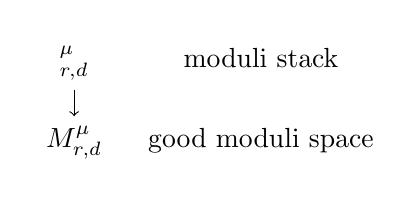
\begin{tikzpicture}
        \matrix (m) [matrix of math nodes, row sep=1em, column sep=1em]
        { \sM^\mu_{r, d} & \text{moduli stack} \\ 
        M^\mu_{r, d} & \text{good moduli space} \\};
        \path[->]
        (m-1-1) edge node[auto,swap] {$  $} (m-2-1)
        ;
        \end{tikzpicture}
        \end{center}
        \item<9-> \textbf{Good moduli space}: parameterizes S-equivalence classes $\leftrightarrow$ polystable sheaves of rank $r$, degree $d$.
        \item<10-> Stack-theoretic techniques $\Rightarrow M^\mu_{r,d}$ exists as a proper algebraic space.
    \end{itemize}
\end{columns}
\end{frame}

\subsection{Projectivity via a determinantal line bundle}
\begin{frame}[fragile]{Dim 1: Projectivity via a determinantal line bundle}
\begin{columns}[t]
    \column{0.5\textwidth}
    \begin{itemize}
        %\item<2-> $\sM^{\text{ss}}_{r,d}$ - stack of semistable vector bundles of $\rk r, \deg d$ on $C$
        %\item<3-> Stack-theoretic techniques $\Rightarrow$ $\sM^{\text{ss}}_{r,d}$ has a \textbf{good moduli space} $M^{\text{ss}}_{r,d}$ as a proper algebraic space.
        \item[]<1-> \textbf{Question}: Is $M^\mu_{r,d}$ projective?
        \item[]<2-> {\footnotesize (Mumford: Yes, using GIT.)}
        \item<3-> Faltings: Ample determinantal line bundle.
        \item<4-> $\sE$ - universal bundle on $\sM^\mu_{r,d} \times C$
        \item[]<5->
        \begin{center}
        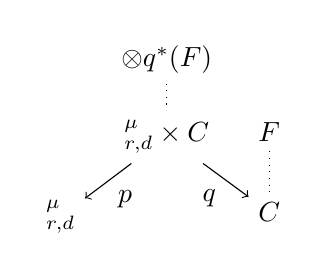
\begin{tikzpicture}
        \matrix (m) [matrix of math nodes, row sep=1em, column sep=1em]
        { & \sE \otimes q^*(F) & \\ 
        & \sM^\mu_{r,d} \times C & F \\
        \sM^\mu_{r,d} & & C \\};
        \path[dotted,-]
        (m-1-2) edge node[auto,swap] {$  $} (m-2-2)
        (m-2-3) edge node[auto,swap] {$  $} (m-3-3)
        ;
        \path[->] 
        (m-2-2) edge node[auto] {$ p $} (m-3-1)
        (m-2-2) edge node[auto,swap] {$ q $} (m-3-3)
        ;
        \end{tikzpicture}
        \end{center}
        \item<5-> For $F \in \Coh(C)$ locally free, set %For $r' \in \N, L \in \Pic(C)$, set
        \[ \la_\sE(F) = \det(R p_* (\sE \otimes q^*F))^\vee. \]
        %if $\rk(F) = r', \det(F) = L$.
        \item<6-> \textit{Depends only on} $\rk(F), \det(F)$.
        \item<7-> Fix $\rk(F), \det(F)$ so that
        \[ \chi(C, E \otimes F) = 0 \text{ for } E \in \sM^\mu_{r,d}. \]
    \end{itemize}
    \pause
    
    \column{0.5\textwidth}
    \begin{itemize}
        \item<8-> (1) $\la_\sE(F)$ descends to $M^\mu_{r,d}$. \\ (2) $R p_* (\sE \otimes q^*F)$ is a 2-term complex
        \[ [\sG_0 \xrightarrow{g} \sG_1], \quad \rk(\sG_0) = \rk(\sG_1). \]
        \item[]<9-> Global section of $\la_\sE(F)$: $s_F = \det(g): \Oh \to \det(\sG_1) \otimes \det(\sG_0)^\vee$
        \item<10-> Vary $F$ with fixed $\rk(F), \det(F)$ $\Rightarrow$ \textit{vary the section} $s_F$.
        \item<11-> \textbf{Thm} (\textit{Faltings 1}): For $E \in \sM^\mu_{r,d}$ $\exists$ $F$ s.t.
        \[ H^0(X, E \otimes F) = H^1(X, E \otimes F) = 0 \]
        \onslide<12->{i.e. $s_F(E) \neq 0$ \pause $\Rightarrow$ $\la_\sE(F)$ is globally generated.}
        %\item<12-> \textbf{Thm} (Faltings): Given $C' \xrightarrow{\sE'} \sM^{\text{ss}}_{r,d}$, if $\deg(\la_\sE(r',L)|_{C'}) = 0$, then $\sE'$ is a family of S-equiv. sheaves. \\ \onslide<13->{$\Rightarrow$ Induced map $M^{\text{ss}}_{r,d} \to \p^N$ is finite, i.e. $\la_\sE(r',L)$ is ample.}
        \item<13-> \textbf{Thm} (\textit{Faltings 2}): $\la_\sE(F)$ is \textit{strictly nef}: $\deg(\la_\sE(F)|_{C'}) > 0$ for any $C' \subs M^\mu_{r,d}$.
        \item[]<14->$\Rightarrow$ Induced map $M^\mu_{r,d} \to \p^N$ is finite, so $\la_\sE(F)$ is ample.
    \end{itemize}
\end{columns}
\end{frame}

\section{Dimension 2}
\subsection{Gieseker and Uhlenbeck moduli spaces}
\begin{frame}[fragile]{Dim 2: Gieseker and Uhlenbeck moduli spaces}
    \begin{itemize}
        \item<2->[] $X$ smooth, projective surface, $H \subs X$ very ample divisor
        \item<3->[] $v \in \Kn(X)$ class with $\rk(v) > 0$
        \item[]
    \end{itemize}
    
    \begin{columns}[t]
        \column{0.5\textwidth}
        \onslide<4->{\textbf{Gieseker stability}}
        \begin{itemize}
            \item<5-> Define stability using \textbf{reduced Hilbert polynomial}
            \[ p_E(n) = \frac{1}{\rk(E)} \chi(X, E(n H)) \]
            %\item<6-> HN- and JH-filtrations exist
            \item<6-> Good moduli space $M^{\text{Gies}}_v$ exists as a projective variety - constructed using GIT.
            \item<7-> $M^{\text{Gies}}_v$ parameterizes polystable sheaves -- torsion-free but not necessarily locally free.
            \item[]
            \item[]<14->
            \begin{center}
            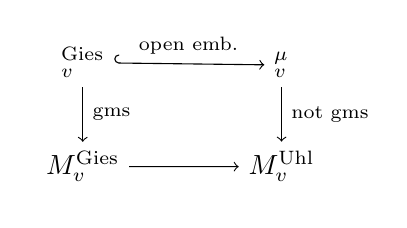
\begin{tikzpicture}
            \matrix (m) [matrix of math nodes, row sep=2em, column sep=4em]
            { \sM^{\mathrm{Gies}}_v & \sM^{\mu}_v \\
            M^{\mathrm{Gies}}_v & M^{\mathrm{Uhl}}_v \\};
            \path[right hook->] 
            (m-1-1) edge node[auto] {$ _\text{open emb.} $} (m-1-2)
            ;
            \path[->]
            (m-1-1) edge node[auto] {$ _\text{gms} $} (m-2-1)
            (m-1-2) edge node[auto] {$ _\text{not gms} $} (m-2-2)
            (m-2-1) edge node[auto] {$  $} (m-2-2)
            ;
            \end{tikzpicture}
            \end{center}
        \end{itemize}
        
        \column{0.5\textwidth}
        \onslide<4->{$\mu$-\textbf{stability}}
        \begin{itemize}
            \item<8-> Define stability using $H$-\textbf{slope}
            \[ \mu(E) = \frac{H \cdot c_1(E)}{\rk(E)} \]
            %\item<10-> HN- and JH-filtrations exist
            \item<9-> No good moduli space in general, but \textbf{Uhlenbeck compactification} comes close:
            \item<10-> $\mu$-semistable sheaves are torsion-free \\
            $\Rightarrow$ \quad $0 \to E \to E^{\vee\vee} \to Q \to 0$ \; with \\ \qquad \; $\dim(Q) = 0$
            \item[]
            \item[]<11-> \textbf{Thm} (J. Li): Projective scheme $M^{\text{Uhl}}_v$ param. $\mu$-polystable sheaves up to:
            \begin{enumerate}
                \item<12-> isomorphic $E^{\vee\vee}$ 
                \item<13-> equal $l_p(Q)$ for all $p \in X$
            \end{enumerate}
        \end{itemize}
    \end{columns}
\end{frame}

\subsection{Bridgeland stability}
\begin{frame}{Dim 2: Bridgeland stability}
    \begin{columns}[t]
        \column{0.5\textwidth}
        \textbf{Fundamentals}
        \begin{itemize}
            %\item<2-> $X$ a smooth, projective variety
            \item<2-> Bridgeland (2003): generalize stability from $\Coh(X)$ to $D^b(X)$.
            \item<3-> A \textbf{stability condition} is $\si = (\sA, Z)$:
            \begin{itemize}
                \item<4-> $\sA \subs D^b(X)$ heart of a t-structure \\
                \qquad\qquad (full abelian subcategory)
                \item<5-> $Z: \Kn(X) \to \C$ group hom.
                \item<6-> $Z(\sA) \subset \Hb = \{ z \;|\; 0 < \arg(z) \le \pi \}$
            \end{itemize}
            \item<7-> $E \in \sA$ is \textbf{semistable} if for subobjects $F \subs E$,
            \[ \arg(Z(F)) \le \arg(Z(E)). \]
            \item<8-> \textbf{Thm} (Bridgeland): Stability conditions parameterized by a \textit{complex manifold} $\Stab(X)$. For fixed $v \in \Kn(X)$, wall-and-chamber structure on $\Stab(X)$.
            %\item<10-> If $\dim X = 1$, then $(\Coh(X), -\deg + i \rk) \in \Stab(X)$.
            %\item<11-> No $Z$ for $\sA = \Coh(X)$ if $\dim X \ge 2$.
            \item<9-> Existence is nontrivial -- $\Coh(X)$ doesn't work as $\sA$.
        \end{itemize}
        
        \column{0.5\textwidth}
        \textbf{Construction of stability conditions}
        \begin{itemize}
            %\item<12-> $(X,H)$ smooth, proj., polarized surface, $v \in \Kn(X)$
            \item<10-> Construct $\sA$ by \textit{tilting} $\Coh(X)$: % with \\ respect to $\mu$
            write $\Coh(X) = \langle \sT, \sF \rangle$, set $\sA = \langle \sF, \sT[-1] \rangle$.
            \item<11-> For $\al, \be \in \R, \al > 0$, set
            \begin{align*}
                Z_{\al, \be}(E) & = \int_X e^{-(\al + \be i)H}\ch(E) \\
                \sA_\be & = \{ E \;|\; F \to E \to T[-1] \}
            \end{align*}
            where $F, T \in \Coh(X), \mu(F) \le \be < \mu(T)$. %$F, T \in \Coh(X)$ s.t. HN-factors satisfy $\mu(F_i) \le \be, \; \mu(T_i) > \be$.
            \item<11-> \textbf{Thm} (B, A--B): $(\sA_\be, Z_{\al,\be}) \in \Stab(X)$.
            \item[]<12->
            \begin{center}
        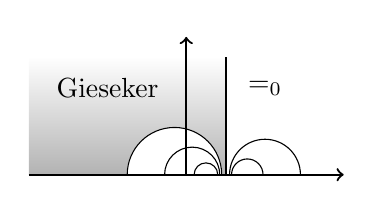
\begin{tikzpicture}[scale=0.5]

        \shadedraw[bottom color=black!30!white,top color=white,draw=white] (-4,0) -- (-1.5,0) arc (180:0:1.2) -- (0,0) -- (1,0) -- (1,3) -- (-4,3);

        \draw[thick,->] (-4,0) -- (4,0) node[anchor=south east] {$\be$};
        \draw[thick,->] (0,0) -- (0,3.5) node[anchor=west] {$\al$};
        \draw[thick] (1,0) -- (1,3);

        \draw[] (0.9,0) arc (0:180:1.2);
        \draw[] (0.85,0) arc (0:180:0.7);
        \draw[] (0.8,0) arc (0:180:0.3);
        \draw[] (1.1,0) arc (180:0:0.9);
        \draw[] (1.15,0) arc (180:0:0.4);

        \draw (-2,2.2) node {Gieseker};
        \draw (2,2.2) node {$\be = \be_0$};

        \end{tikzpicture}
        \end{center}
            \item<13-> \textbf{Thm} (T, A--HL--H): Moduli stack $\sM^\si_v$ is algebraic, of finite type, universally closed, good moduli space $M^\si_v$ is a \textit{proper algebraic space}.
        \end{itemize}
    \end{columns}
\end{frame}

\subsection{{\color{purple} Projectivity on vertical wall \& Uhlenbeck}}
\begin{frame}[fragile]{Dim 2: Projectivity, vertical wall, and Uhlenbeck}
    \begin{columns}[t]
        \column{0.5\textwidth}
        \onslide<1->{\textbf{Question}: Is $M^\si_v$ projective?}
        \begin{itemize}
            \item<2-> Previously know cases (incomplete list):
            \begin{itemize}
                \item<3-> $X = \p^2$ {\footnotesize (ABCH)}, $\p^1 \times \p^1, \text{Bl}_p \p^2$ {\footnotesize (AM)} - exceptional collections and quiver GIT.
                \item<4-> Gieseker stability for any $X$. {\footnotesize (B)}
                \item<5-> $X = $ K3 {\footnotesize (BM)} or Enriques {\footnotesize (N)}: relate to Gieseker by Fourier-Mukai.
            \end{itemize}
        \item<6-> \textbf{Thm} (B--M): (cf. \textit{Faltings 2}) Determinantal line bundle $\sL_\si$ that is \textit{strictly nef} on $M^\si_v$: %$\exists \; w_\si \in K(X)$ s.t. $\sL_\si = \la_\sE(w_\si)$ 
        \item[]<6-> $\deg(\sL_\si|_C) > 0$ for $C \subs M^\si_v$.
        \item<7-> $\Rightarrow$ If some $\sL_\si^{\otimes n}$ is globally generated, then $\sL_\si$ is ample!
        \item[]
        \item[]<8->
        \begin{center}
        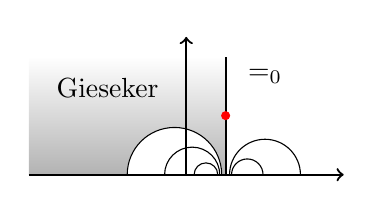
\begin{tikzpicture}[scale=0.5]

        \shadedraw[bottom color=black!30!white,top color=white,draw=white] (-4,0) -- (-1.5,0) arc (180:0:1.2) -- (0,0) -- (1,0) -- (1,3) -- (-4,3);

        \draw[thick,->] (-4,0) -- (4,0) node[anchor=south east] {$\be$};
        \draw[thick,->] (0,0) -- (0,3.5) node[anchor=west] {$\al$};
        \draw[thick] (1,0) -- (1,3);

        \draw[] (0.9,0) arc (0:180:1.2);
        \draw[] (0.85,0) arc (0:180:0.7);
        \draw[] (0.8,0) arc (0:180:0.3);
        \draw[] (1.1,0) arc (180:0:0.9);
        \draw[] (1.15,0) arc (180:0:0.4);

        \draw (-2,2.2) node {Gieseker};
        \draw (2,2.5) node {$\be = \be_0$};
        \draw [red,fill] (1,1.5) circle [radius=0.1] node[black,anchor=west] {$\si$};

        \end{tikzpicture}
        \end{center}
        \end{itemize}
                
        \column{0.5\textwidth}
        \onslide<8->{\textbf{New affirmative case}: vertical wall}
        \begin{itemize}
            %\item<9-> $(\al,\be)$-plane contains \textit{Gieseker chamber}, bounded by \textit{vertical wall} $\be = \be_0$.
            \item<9-> Polystable objects: $F \oplus (\oplus_i \Oh_{p_i}[-1])$, \\ $F$ $\mu$-polystable \textit{locally free}, and $p_i \in X$ \\ $\Rightarrow$ set-theoretic bijection with $M^{\text{Uhl}}_v$ (L--Q).
            \item<10-> Uhlenbeck-equiv. becomes \textit{S-equiv. for} $\si$: If $E \in \Coh(X)$ is $\mu$-stable but \textit{not locally free}, rotate $0 \to E \to E^{\vee\vee} \to Q \to 0$
            \begin{align*}
                \Rightarrow \quad E \; & \overset{\text{S}}{\sim} \; E^{\vee\vee} \oplus Q[-1] \\
                & \overset{\text{S}}{\sim} \; E^{\vee\vee} \oplus \bigoplus_{p \in X} \Oh_p^{\oplus l_p(Q)}[-1]
            \end{align*} 
            \item[]<11-> \underline{\textbf{Thm} (T)}: On vertical wall:
            %\begin{itemize}
                \item[]<12-> $\sL_\si$ is ample and $M^\si_v$ is projective.
                \item[]<13-> Bijective morphism $M^{\text{Uhl}}_v \to M^\si_v$.
            %\end{itemize}
            
            \item[]
            \item[]<14->
            \begin{center}
            \begin{tikzpicture}
            \matrix (m) [matrix of math nodes, row sep=2em, column sep=2em]
            { \sM^{\mathrm{Gies}}_v & \sM^{\mu}_v & \sM^\si_v \\
            M^{\mathrm{Gies}}_v & M^{\mathrm{Uhl}}_v & M^\si_v \\};
            \path[right hook->] 
            (m-1-1) edge node[auto] {$ _\text{open} $} (m-1-2)
            (m-1-2) edge node[auto] {$ _\text{open} $} (m-1-3)
            ;
            \path[->]
            (m-1-1) edge node[auto] {$ _\text{gms} $} (m-2-1)
            (m-1-2) edge node[auto] {$ $} (m-2-2)
            (m-1-3) edge node[auto,swap] {$ _\text{gms} $} (m-2-3)
            (m-2-1) edge node[auto] {$ $} (m-2-2)
            (m-2-2) edge node[auto] {$ _\text{bij.} $} (m-2-3)
            ;
            \end{tikzpicture}
            \end{center}
        \end{itemize}
    \end{columns}
\end{frame}

\subsection{Proof sketch \& questions}
\begin{frame}[fragile]{Dim 2: Proof sketch \& questions}
    \begin{columns}[t]
        \column{0.5\textwidth}
        \textbf{Proof sketch}
        \begin{itemize}
            \item<2-> Special to vertical wall: there are curves $C \in |m H|$ and $F \in \Coh(C)$ s.t. $\sL_\si^{\otimes n} \cong \la_{j^* \sE}(F)^\vee = \det(R p_*(j^*\sE \otimes q_C^*F))^\vee$.
            %\item[]<3->
            %\begin{center}
            \begin{tikzpicture}
            \matrix (m) [matrix of math nodes, row sep=1em, column sep=1.5em]
            { & \sE & j^* \sE \\ 
            & \sM^\si_v \times X & \sM^\si_v \times C \\
            \sM^\si_v & X & C \\};
            \path[dotted,-]
            (m-1-2) edge node[auto,swap] {$  $} (m-2-2)
            (m-1-3) edge node[auto,swap] {$  $} (m-2-3)
            ;
            \path[left hook->]
            (m-2-3) edge node[auto] {$ j $} (m-2-2)
            (m-3-3) edge node[auto] {$ $} (m-3-2)
            ;
            \path[->] 
            (m-2-2) edge node[auto,swap] {$ p $} (m-3-1)
            (m-2-2) edge node[auto] {$ $} (m-3-2)
            (m-2-3) edge node[auto] {$ q_C $} (m-3-3)
            ;
            \end{tikzpicture}
            %\end{center}
            \item<3-> Strategy: restriction to $C$ \& \textit{Faltings 1}.
            \item<4-> \textbf{Lemma 1}: for any $E \in \sM^\si_v$ and $C \in |m H|$,
            $H^i(C, F \otimes E|_C) = 0$ for $i \neq 0, 1$,
            \[ \dim H^0(C, F \otimes E|_C) = \dim H^1(C, F \otimes E|_C) \]
            $\Rightarrow$ $\la_{j^*\sE}(F)^\vee = \det[\sG_0 \xrightarrow{g} \sG_1]$ has section $s_F = \det(g)$.
            \item<5-> %$\sM^\si_v$ quasi-comp. \& $\sL_\si$ strictly nef \\ $\Rightarrow$ 
            Enough to show: for $[E_0] \in \sM^\si_v$ there is $F$ with $s_F(E_0) \neq 0$.
        \end{itemize}
        
        \column{0.5\textwidth}
        \begin{itemize}
            \item<6-> \textbf{Thm} (F): If $F \in \Coh(X)$ is $\mu$-semistable, for generic $C \in |m H|$, restriction $F|_C$ is semistable.
            \item<7-> \textbf{Lemma 2}: For generic $C \in |m H|$, restriction $E_0|_C$ is a semistable sheaf.
            \item<8-> Apply \textit{Faltings 1}: choose $F \in \Coh(C)$ s.t. 
            \[ H^0(C, F \otimes E_0|_C) = H^1(C, F \otimes E_0|_C) = 0 \]
            $\Rightarrow$ $s_F(E_0) \neq 0$.
            \item<9-> $M^{\text{Uhl}}_v \to M^\si_v$ for free from Li's construction.
        \end{itemize}
        \onslide<10->{\textbf{Questions}}
        \begin{itemize}
            \item<11-> Is $M^{\text{Uhl}}_v \to M^\si_v$ isomorphism? \\ {\footnotesize (Could have different singularities/non-reduced structure.)}
            \item<12-> Projectivity of other Bridgeland moduli spaces? For starters, is $\sL_{\si_\text{Gies}}$ relatively ample for $M^{\text{Gies}}_v \to M^\si_v$?
            \item<13-> Projectivity of other moduli of sheaves or complexes when GIT isn't available?
        \end{itemize}
    \end{columns}
\end{frame}

\section{Dimension 3}
\subsection{Work in progress: PT-stability}
\begin{frame}{Dim 3: PT-stability (work in progress)}
    \begin{itemize}
        \item[]<2-> $X$ smooth, projective 3-fold, $H \subs X$ very ample
        \item[]<2-> $v \in \Kn(X)$ with $\rk(v) > 0$
    \end{itemize}
    
    \begin{columns}[t]
        \column{0.5\textwidth}
        \begin{itemize}
            \item<3-> A \textbf{PT-stable pair} is
            \[ \Oh_X \xrightarrow{f} F, \]
            $F$ pure dim 1, $\dim(\coker(f)) = 0$.
            \item<4-> (Bayer, Toda) Higher rank PT-pairs from \textit{polynomial/limit stability}.
            \item<5-> Heart of ``perverse sheaves'' $\sA^p \subs D^b(X)$ , $Z: \Kn(X) \to \C[t]$.
            \item<5-> Stability on $\sA^p$ using $\arg(Z(E))$ for $t \gg 0$.
            \item<6-> PT-semistable $E \in \sA^p$ satisfies
            \begin{itemize}
                \item<7-> $\sH^0(E)$ is $\mu$-semistable
                \item<7-> $\sH^1(E)$ is 0-dimensional
                \item<8-> $\Hom(T[-1], E) = 0$ if $\dim(T) = 0$
            \end{itemize}
            \item<9-> \textbf{Thm} (Lo): Moduli stack $\sM^{\text{PT}}_v$ is algebraic, of finite type, universally closed.
        \end{itemize}
        
        \column{0.5\textwidth}
        \begin{itemize}
            \item[]<10-> \underline{\textbf{Thm(ish)} (T)}: 
            %\begin{itemize}
                \item[]<11-> A determinantal line bundle $\sL$ on $\sM^{\text{PT}}_v$ is globally generated.
                \item[]<12-> Induced morphism $\pi: \sM^{\text{PT}}_v \to \p^N$ is injective on the locus of $\mu$-stable vector bundles.
            %\end{itemize}
            \item[]
            \item<13-> Global generation follows by restricting to curves.
            \item<14-> Questions:
            \begin{itemize}
                \item<15-> Does $\sM^{\text{PT}}_v$ have a good moduli space? Is it projective?
                \item<16-> What are fibers of $\pi$?
                \item<17-> Image of $\pi$ = analog of Uhlenbeck compactification for a 3-fold?
            \end{itemize}
            
        \end{itemize}
    \end{columns}
\end{frame}

\end{document}